\documentclass[aspectratio=169]{beamer}

\usepackage[T5]{fontenc}
\usepackage[utf8]{inputenc}
\usepackage{lmodern}

\usetheme{Madrid}

\usepackage{graphicx}
\usepackage{multicol}
\usepackage{amsmath,amssymb}

% Outline look: blue text, numbered, no balls
\setbeamertemplate{section in toc}{%
  \leavevmode\inserttocsectionnumber.~\inserttocsection\par}
\setbeamercolor{section in toc}{fg=blue}

\hypersetup{colorlinks=true, urlcolor=blue}

\newcommand{\backbtn}{%
  \hfill\hyperlink{outline}{\beamerbutton{Mục lục}}}


% Giảm khoảng cách trên/dưới công thức hiển thị để slide gọn hơn
\makeatletter
\def\tight@disp{\setlength\abovedisplayskip{4pt plus 2pt}%
  \setlength\belowdisplayskip{4pt plus 2pt}%
  \setlength\abovedisplayshortskip{2pt plus 1pt}%
  \setlength\belowdisplayshortskip{2pt plus 1pt}}
\g@addto@macro\normalsize{\tight@disp}
\g@addto@macro\small{\tight@disp}
\g@addto@macro\footnotesize{\tight@disp}
\g@addto@macro\scriptsize{\tight@disp}
\makeatother

\title[Ứng suất chính]{Ứng suất chính dưới tác dụng của tải trọng cho trước}
\author[© N. V. Sỹ]{Nguyễn Văn Sỹ}
\institute[TNUT]{%
  Bộ môn Hệ thống Công nghiệp \\
  Trường Đại học Kỹ thuật Công nghiệp \\
  \href{mailto:vansy@tnut.edu.vn}{vansy@tnut.edu.vn}}
\date[Cơ học vật liệu]{\large Cơ học vật liệu – Ứng suất chính \\[0.5em] \footnotesize \copyright\ Nguyễn Văn Sỹ}

\begin{document}

\begin{frame}
  \titlepage
\end{frame}
%====================
\begin{frame}{Tài liệu tham khảo}
	\small
	F. P. Beer, E. R. Johnston, Jr., J. T. DeWolf, D. F. Mazurek,
	\emph{Mechanics of Materials}, 6th ed., McGraw-Hill, New York, 2012.
	
	\vspace{1em}
	\footnotesize\color{gray}
	Toàn bộ hình vẽ trong bài giảng được trích từ giáo trình trên, chỉ sử dụng
	cho mục đích giảng dạy nội bộ.
\end{frame}
% ===== OUTLINE SLIDE =====
\begin{frame}[t]{Nội dung}
  \hypertarget{outline}{}
  \scriptsize
  \begin{multicols}{2}
    \tableofcontents[hideallsubsections]
  \end{multicols}
\end{frame}

% ===== CONTENT SLIDES =====
\section{Giới thiệu}
\begin{frame}[t]{Giới thiệu}
  \small
  \begin{itemize}
    \setlength{\itemsep}{0.6em}
    \item Trong Chương 1 và 2, ta đã học cách xác định ứng suất pháp do tải
          trọng đúng tâm.
    \item Trong Chương 3, ta đã phân tích phân bố ứng suất tiếp trong cấu
          kiện tròn chịu ngẫu lực xoắn.
    \item Trong Chương 4, ta đã xác định ứng suất pháp do các ngẫu lực uốn.
    \item Trong Chương 5 và 6, ta đã tính ứng suất tiếp do tải trọng ngang.
    \item Trong Chương 7, ta đã học cách các thành phần ứng suất biến đổi khi
          xoay hệ trục tọa độ và cách xác định các mặt chính, ứng suất chính và
          ứng suất tiếp lớn nhất tại một điểm.
    \item Trong Chương 8, ta sẽ học cách xác định ứng suất trong cấu kiện kết
          cấu hoặc chi tiết máy do tổ hợp tải trọng gây ra, và cách tìm các ứng
          suất chính và ứng suất tiếp lớn nhất tương ứng.
  \end{itemize}
\end{frame}
% ===========
\section{Ứng suất chính trong dầm}
\begin{frame}[t]{Ứng suất chính trong dầm}
  \begin{columns}[T]
    \column{0.56\textwidth}
      \small
      \begin{itemize}
        \setlength{\itemsep}{0.6em}
        \item Dầm lăng trụ chịu tải trọng ngang:
        \[
          \sigma_x = -\frac{My}{I} \qquad \sigma_m = \frac{Mc}{I}
        \]
        \[
          \tau_{xy} = -\frac{VQ}{It} \qquad \tau_m = \frac{VQ}{It}
        \]
        \item Các ứng suất chính được xác định bằng các phương pháp của
              Chương 7.
        \item Liệu ứng suất pháp lớn nhất trên mặt cắt có thể lớn hơn
              \[
                \sigma_m = \frac{Mc}{I}\ ?
              \]
      \end{itemize}
    \column{0.42\textwidth}
      \centering
      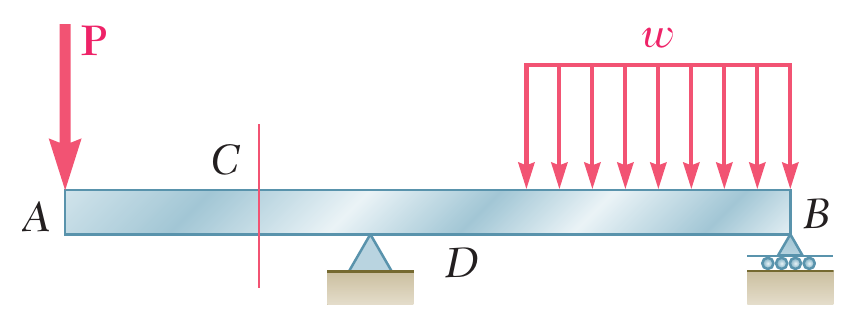
\includegraphics[width=\linewidth,height=5.5cm,keepaspectratio]{Chap_8/fig_8_4.png}
  \end{columns}
\end{frame}
% ===========
\begin{frame}[t]{Ứng suất chính trong dầm (tiếp)}
  \centering
  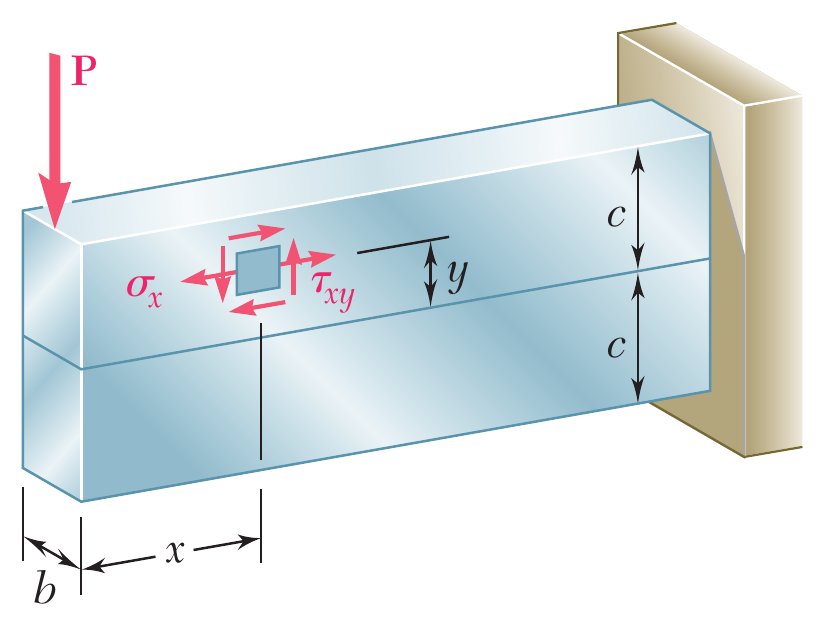
\includegraphics[width=0.32\textwidth,height=2.9cm,keepaspectratio]{Chap_8/fig_8_7.png}\hfill
  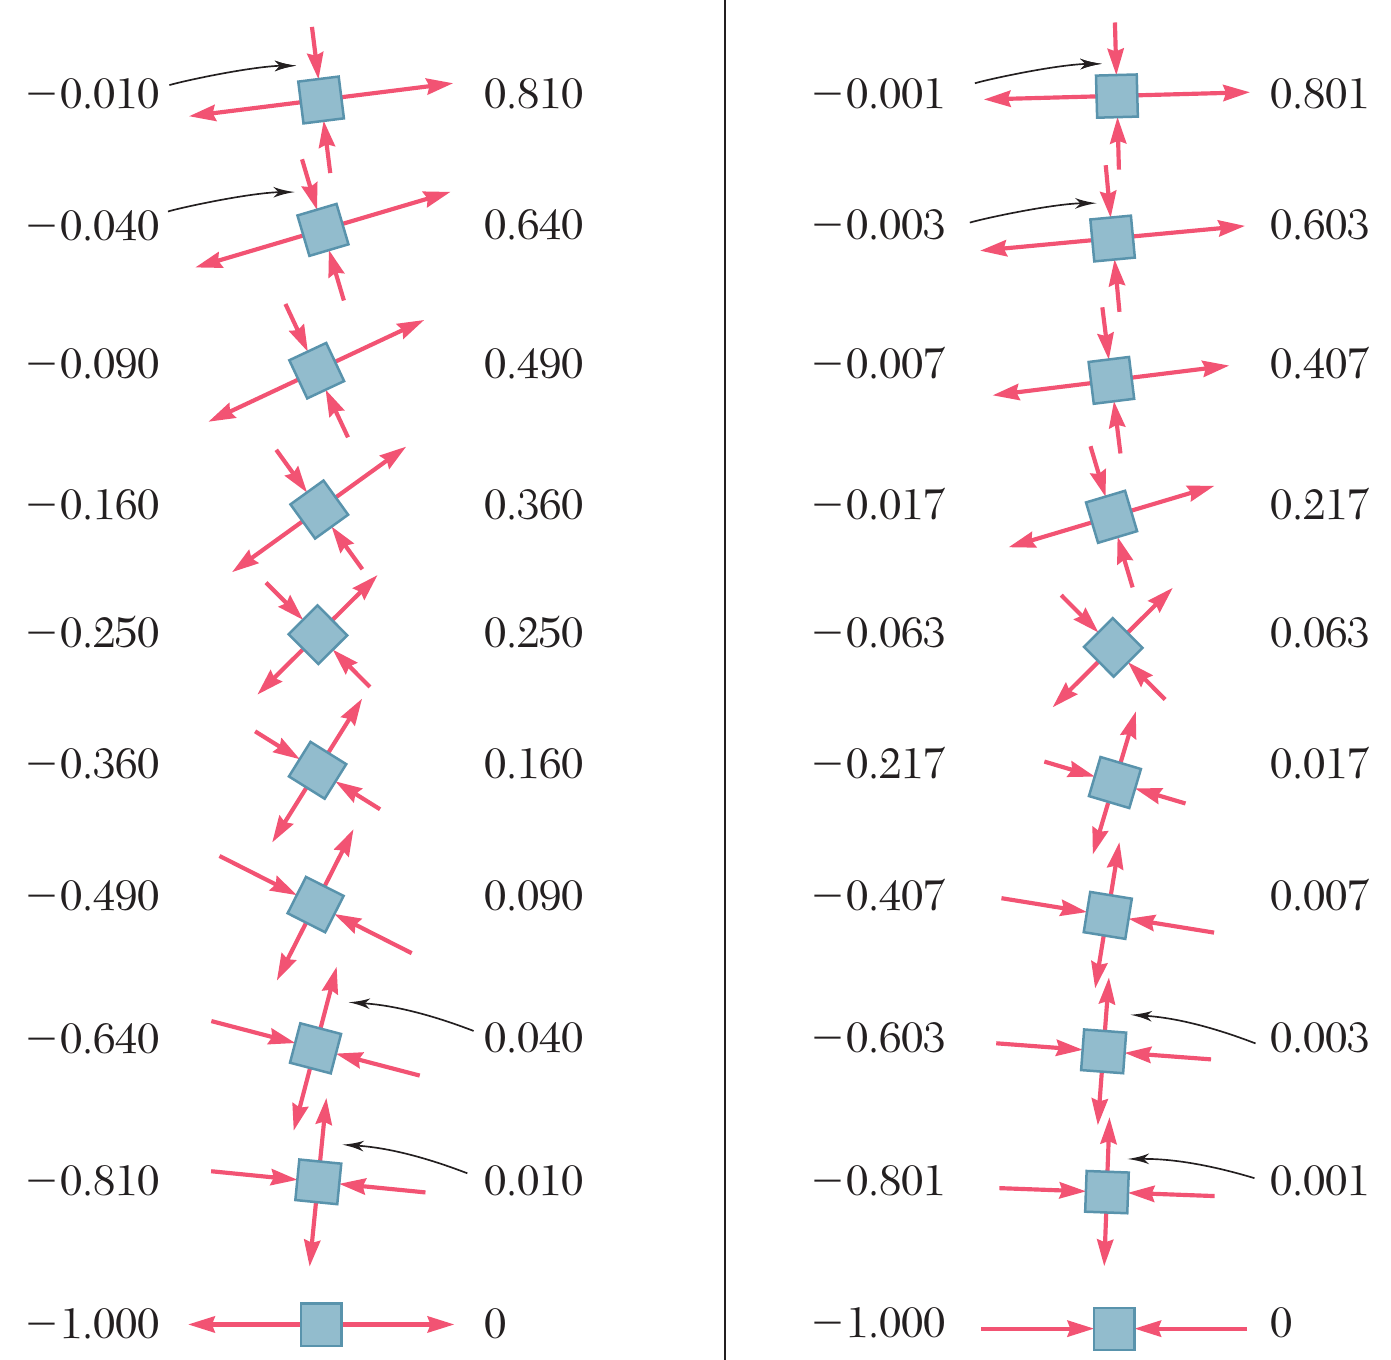
\includegraphics[width=0.32\textwidth,height=2.9cm,keepaspectratio]{Chap_8/fig_8_8.png}\hfill
  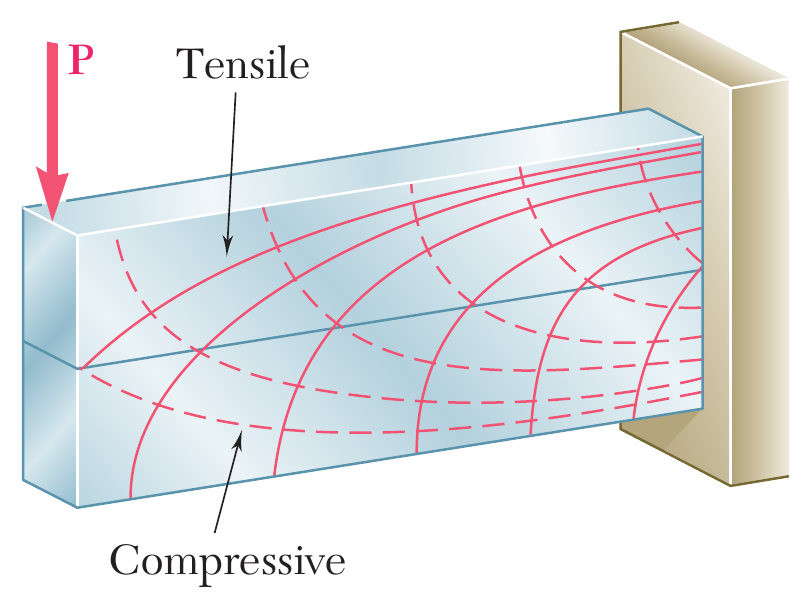
\includegraphics[width=0.32\textwidth,height=2.9cm,keepaspectratio]{Chap_8/fig_8_9.png}\\[6pt]
  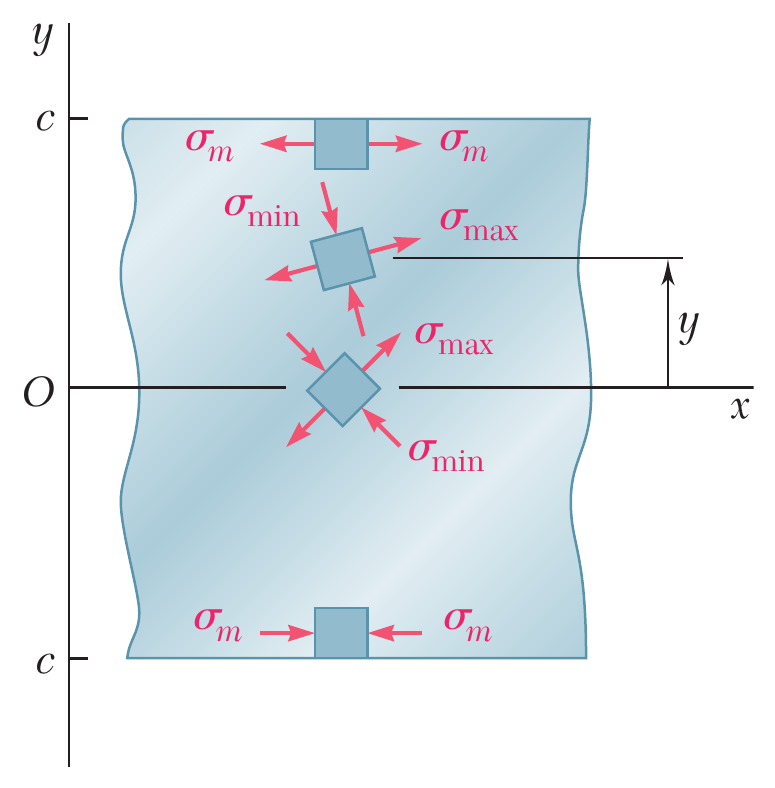
\includegraphics[width=0.6\textwidth,height=2.9cm,keepaspectratio]{Chap_8/fig_8_6.png}
\end{frame}
% ===========
\begin{frame}[t]{Ứng suất chính trong dầm (tiếp)}
  \begin{columns}[T]
    \column{0.48\textwidth}
      \small
      \begin{itemize}
        \setlength{\itemsep}{1em}
        \item Hình dạng mặt cắt ngang dẫn đến giá trị $\tau_{xy}$ lớn ở gần bề
              mặt, nơi $\sigma_x$ cũng lớn.
        \item $\sigma_{\max}$ có thể lớn hơn $\sigma_m$.
      \end{itemize}
    \column{0.50\textwidth}
      \centering
      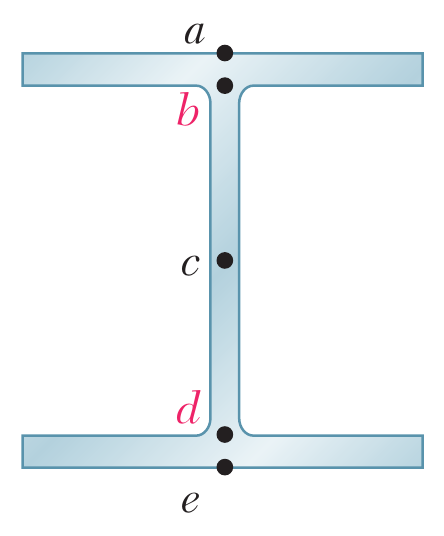
\includegraphics[width=\linewidth,height=5.5cm,keepaspectratio]{Chap_8/fig_8_10.png}
  \end{columns}
\end{frame}
% ===========
\section{Bài mẫu 8.1}
\begin{frame}[t]{Bài mẫu 8.1}
  \begin{columns}[T]
    \column{0.42\textwidth}
      \centering
      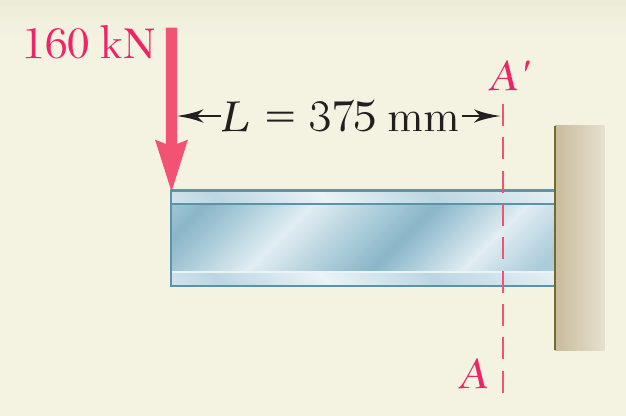
\includegraphics[width=\linewidth,height=5.5cm,keepaspectratio]{Chap_8/sp_8_1_a.png}
    \column{0.56\textwidth}
      \small
      Một lực 160 kN tác dụng tại đầu dầm thép cán W200$\times$52. Bỏ qua ảnh
      hưởng của góc lượn và tập trung ứng suất, xác định xem các ứng suất
      pháp có thỏa mãn yêu cầu thiết kế là không vượt quá 150 MPa tại mặt cắt
      $A$--$A'$ hay không.

      \vspace{0.5em}
      \textbf{LỜI GIẢI:}
      \begin{itemize}
        \setlength{\itemsep}{0.3em}
        \item Xác định lực cắt và mô men uốn tại mặt cắt $A$--$A'$.
        \item Tính ứng suất pháp tại mặt trên và tại chỗ nối cánh -- bụng.
        \item Tính ứng suất tiếp tại chỗ nối cánh -- bụng.
        \item Tính ứng suất chính tại chỗ nối cánh -- bụng.
      \end{itemize}
  \end{columns}
\end{frame}
% ===========
\begin{frame}[t]{Bài mẫu 8.1 (tiếp)}
  \begin{columns}[T]
    \column{0.56\textwidth}
      \small
      \textbf{LỜI GIẢI:}
      \begin{itemize}
        \setlength{\itemsep}{0.6em}
        \item Xác định lực cắt và mô men uốn tại mặt cắt $A$--$A'$:
        \[
          M_A = (160\,\mathrm{kN})(0{,}375\,\mathrm{m}) = 60\,\mathrm{kN\cdot m}
        \]
        \[
          V_A = 160\,\mathrm{kN}
        \]
        \item Tính ứng suất pháp tại mặt trên và tại chỗ nối cánh -- bụng:
        \[
          \sigma_a = \frac{M_A}{S}
            = \frac{60\,\mathrm{kN\cdot m}}{512\times10^{-6}\,\mathrm{m}^3}
            = 117{,}2\,\mathrm{MPa}
        \]
        \[
          \sigma_b = \sigma_a\frac{y_b}{c}
            = (117{,}2\,\mathrm{MPa})\frac{90{,}4\,\mathrm{mm}}{103\,\mathrm{mm}}
            = 102{,}9\,\mathrm{MPa}
        \]
      \end{itemize}
    \column{0.42\textwidth}
      \centering
      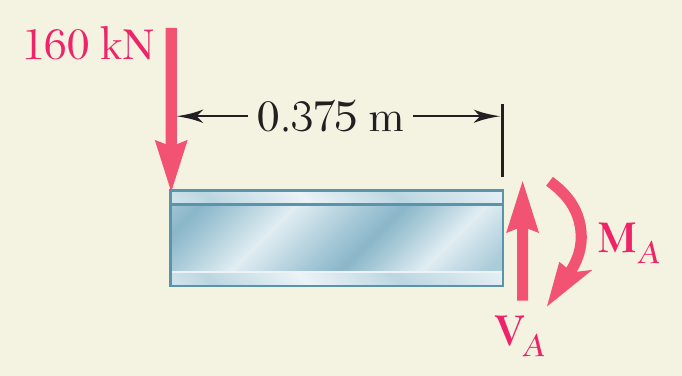
\includegraphics[width=\linewidth,height=5.5cm,keepaspectratio]{Chap_8/sp_8_1_b.png}
  \end{columns}
\end{frame}
% ===========
\begin{frame}[t]{Bài mẫu 8.1 (tiếp)}
  \begin{columns}[T]
    \column{0.58\textwidth}
      \small
      \begin{itemize}
        \setlength{\itemsep}{0.5em}
        \item Tính ứng suất tiếp tại chỗ nối cánh -- bụng:
        \[
          Q = (204\times12{,}6)\,96{,}7 = 248{,}6\times10^{3}\,\mathrm{mm}^3
        \]
        \[
          \tau_b = \frac{V_AQ}{It}
            = \frac{(160\times10^{3})(248{,}6\times10^{-6})}
                   {(52{,}7\times10^{-6})(0{,}0079)}
            = 95{,}5\,\mathrm{MPa}
        \]
        \item Tính ứng suất chính tại chỗ nối cánh -- bụng:
        \[
          \sigma_{\max} = \tfrac{1}{2}\sigma_b
            + \sqrt{\left(\tfrac{1}{2}\sigma_b\right)^2 + \tau_b^2}
        \]
        \[
          \sigma_{\max} = \frac{102{,}9}{2} + \sqrt{\left(\frac{102{,}9}{2}\right)^2 + (95{,}5)^2}
        \]
        \[
          = 159{,}9\,\mathrm{MPa}\ (> 150\,\mathrm{MPa})
        \]
        \alert{Yêu cầu thiết kế không được thỏa mãn.}
      \end{itemize}
    \column{0.40\textwidth}
      \centering
      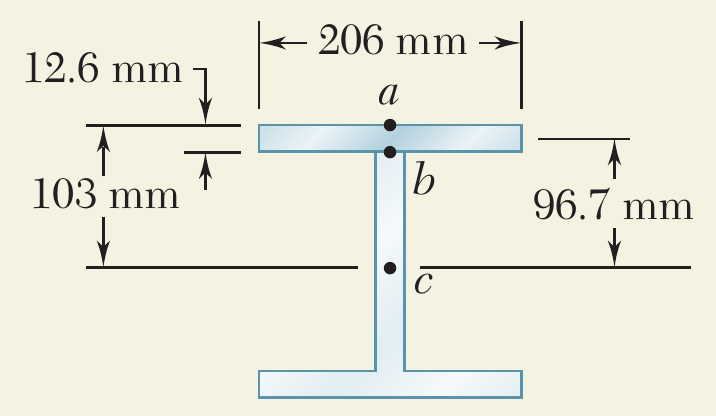
\includegraphics[width=\linewidth,height=5.5cm,keepaspectratio]{Chap_8/sp_8_1_c.png}
  \end{columns}
\end{frame}
% ===========
\section{Bài mẫu 8.2}
\begin{frame}[t]{Bài mẫu 8.2}
  \begin{columns}[T]
    \column{0.42\textwidth}
      \centering
      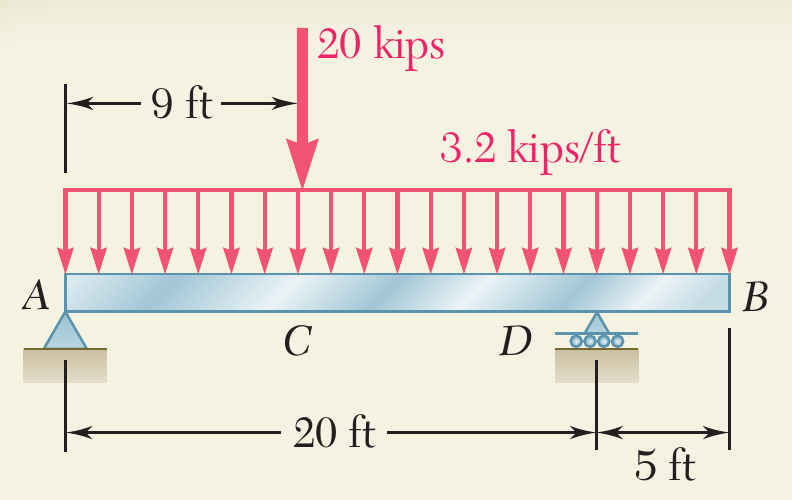
\includegraphics[width=\linewidth,height=5.5cm,keepaspectratio]{Chap_8/sp_8_2_a.png}
    \column{0.56\textwidth}
      \small
      Dầm có đầu thừa chịu tải trọng phân bố đều và một tải trọng tập trung.
      Biết với mác thép sử dụng $\sigma_{\mathrm{all}} = 165\,\mathrm{MPa}$ và
      $\tau_{\mathrm{all}} = 100\,\mathrm{MPa}$, hãy chọn dầm chữ I cánh rộng
      phù hợp.

      \vspace{0.5em}
      \textbf{LỜI GIẢI:}
      \begin{itemize}
        \setlength{\itemsep}{0.3em}
        \item Xác định phản lực tại $A$ và $D$.
        \item Xác định lực cắt và mô men uốn lớn nhất từ các biểu đồ lực cắt
              và mô men uốn.
        \item Tính mô men chống uốn cần thiết và chọn mặt cắt dầm phù hợp.
        \item Tìm ứng suất pháp lớn nhất.
        \item Tìm ứng suất tiếp lớn nhất.
      \end{itemize}
  \end{columns}
\end{frame}
% ===========
\begin{frame}[t]{Bài mẫu 8.2 (tiếp)}
  \begin{columns}[T]
    \column{0.56\textwidth}
      \footnotesize
      \textbf{LỜI GIẢI:}
      \begin{itemize}
        \setlength{\itemsep}{0.25em}
        \item Xác định phản lực tại $A$ và $D$:
        \[
          \textstyle\sum M_A = 0 \;\Rightarrow\; R_D = 265{,}5\,\mathrm{kN}
        \]
        \[
          \textstyle\sum M_D = 0 \;\Rightarrow\; R_A = 184{,}5\,\mathrm{kN}
        \]
        \item Xác định lực cắt và mô men uốn lớn nhất từ các biểu đồ:
        \[
          |M|_{\max} = 323{,}2\,\mathrm{kN\cdot m} \quad\text{với}\quad
          V = 54{,}9\,\mathrm{kN}
        \]
        \[
          |V|_{\max} = 193{,}4\,\mathrm{kN}
        \]
        \item Tính mô men chống uốn cần thiết và chọn mặt cắt dầm phù hợp:
        \[
          S_{\min} = \frac{|M|_{\max}}{\sigma_{\mathrm{all}}}
            = \frac{323\times10^{3}\,\mathrm{N\cdot m}}{165\times10^{6}\,\mathrm{Pa}}
            = 1959\times10^{3}\,\mathrm{mm}^3
        \]
        chọn mặt cắt dầm \textbf{W530$\times$92}
      \end{itemize}
    \column{0.42\textwidth}
      \centering
      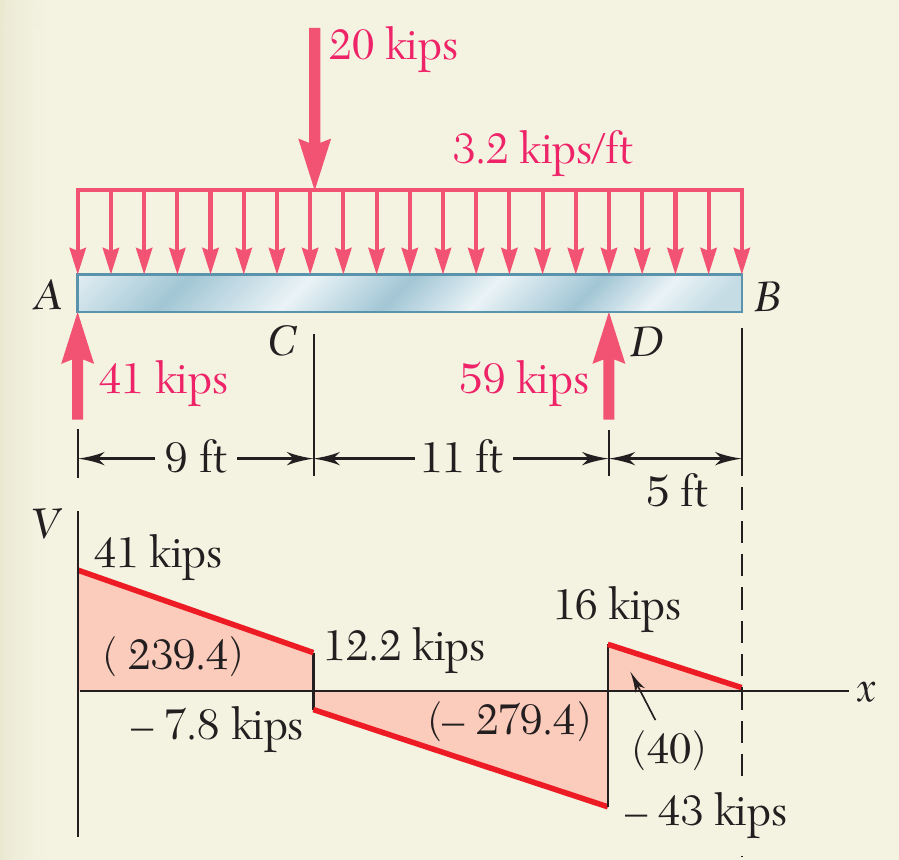
\includegraphics[width=\linewidth,height=4.7cm,keepaspectratio]{Chap_8/sp_8_2_b.png}
  \end{columns}
\end{frame}
% ===========
\begin{frame}[t]{Bài mẫu 8.2 (tiếp)}
  \begin{columns}[T]
    \column{0.60\textwidth}
      \footnotesize
      \begin{itemize}
        \setlength{\itemsep}{0.4em}
        \item Tìm ứng suất tiếp lớn nhất. Giả thiết ứng suất tiếp phân bố đều
              trong bụng dầm:
        \[
          \tau_{\max} = \frac{V_{\max}}{A_{\text{bụng}}}
            = \frac{193{,}4\times10^{3}\,\mathrm{N}}{5436{,}6\times10^{-6}\,\mathrm{m}^2}
            = 35{,}6\,\mathrm{MPa} < 100\,\mathrm{MPa}
        \]
        \item Tìm ứng suất pháp lớn nhất:
        \[
          \sigma_a = \frac{|M|_{\max}}{S}
            = \frac{323\,200\,\mathrm{N\cdot m}}{2{,}07\times10^{-3}\,\mathrm{m}^3}
            = 156{,}1\,\mathrm{MPa}
        \]
        \[
          \sigma_b = \sigma_a\frac{y_b}{c}
            = (156{,}1\,\mathrm{MPa})\frac{250{,}9\,\mathrm{mm}}{266{,}5\,\mathrm{mm}}
            = 147\,\mathrm{MPa}
        \]
        \[
          \tau_b = \frac{V}{A_{\text{bụng}}}
            = \frac{54\,900\,\mathrm{N}}{5436{,}6\times10^{-6}\,\mathrm{m}^2}
            = 10{,}1\,\mathrm{MPa}
        \]
        \[
          \sigma_{\max} = \frac{147\,\mathrm{MPa}}{2}
            + \sqrt{\left(\frac{147\,\mathrm{MPa}}{2}\right)^2 + (10{,}1\,\mathrm{MPa})^2}
        \]
        \[
          \sigma_{\max} = 147{,}1\,\mathrm{MPa} < 165\,\mathrm{MPa}
        \]
      \end{itemize}
    \column{0.38\textwidth}
      \centering
      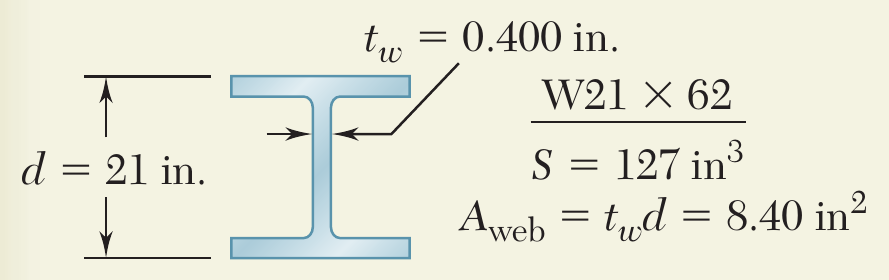
\includegraphics[width=\linewidth,height=5.5cm,keepaspectratio]{Chap_8/sp_8_2_c.png}
  \end{columns}
\end{frame}
% ===========
\section{Thiết kế trục truyền động}
\begin{frame}[t]{Thiết kế trục truyền động}
  \begin{columns}[T]
    \column{0.56\textwidth}
      \small
      \begin{itemize}
        \setlength{\itemsep}{0.8em}
        \item Nếu công suất được truyền vào và ra khỏi trục qua bánh răng hoặc
              đĩa xích, trục chịu tải trọng ngang cũng như tải trọng xoắn.
        \item Ứng suất pháp do tải trọng ngang có thể lớn và cần được kể đến
              khi xác định ứng suất tiếp lớn nhất.
        \item Ứng suất tiếp do tải trọng ngang thường nhỏ và phần đóng góp của
              nó vào ứng suất tiếp lớn nhất có thể bỏ qua.
      \end{itemize}
    \column{0.42\textwidth}
      \centering
      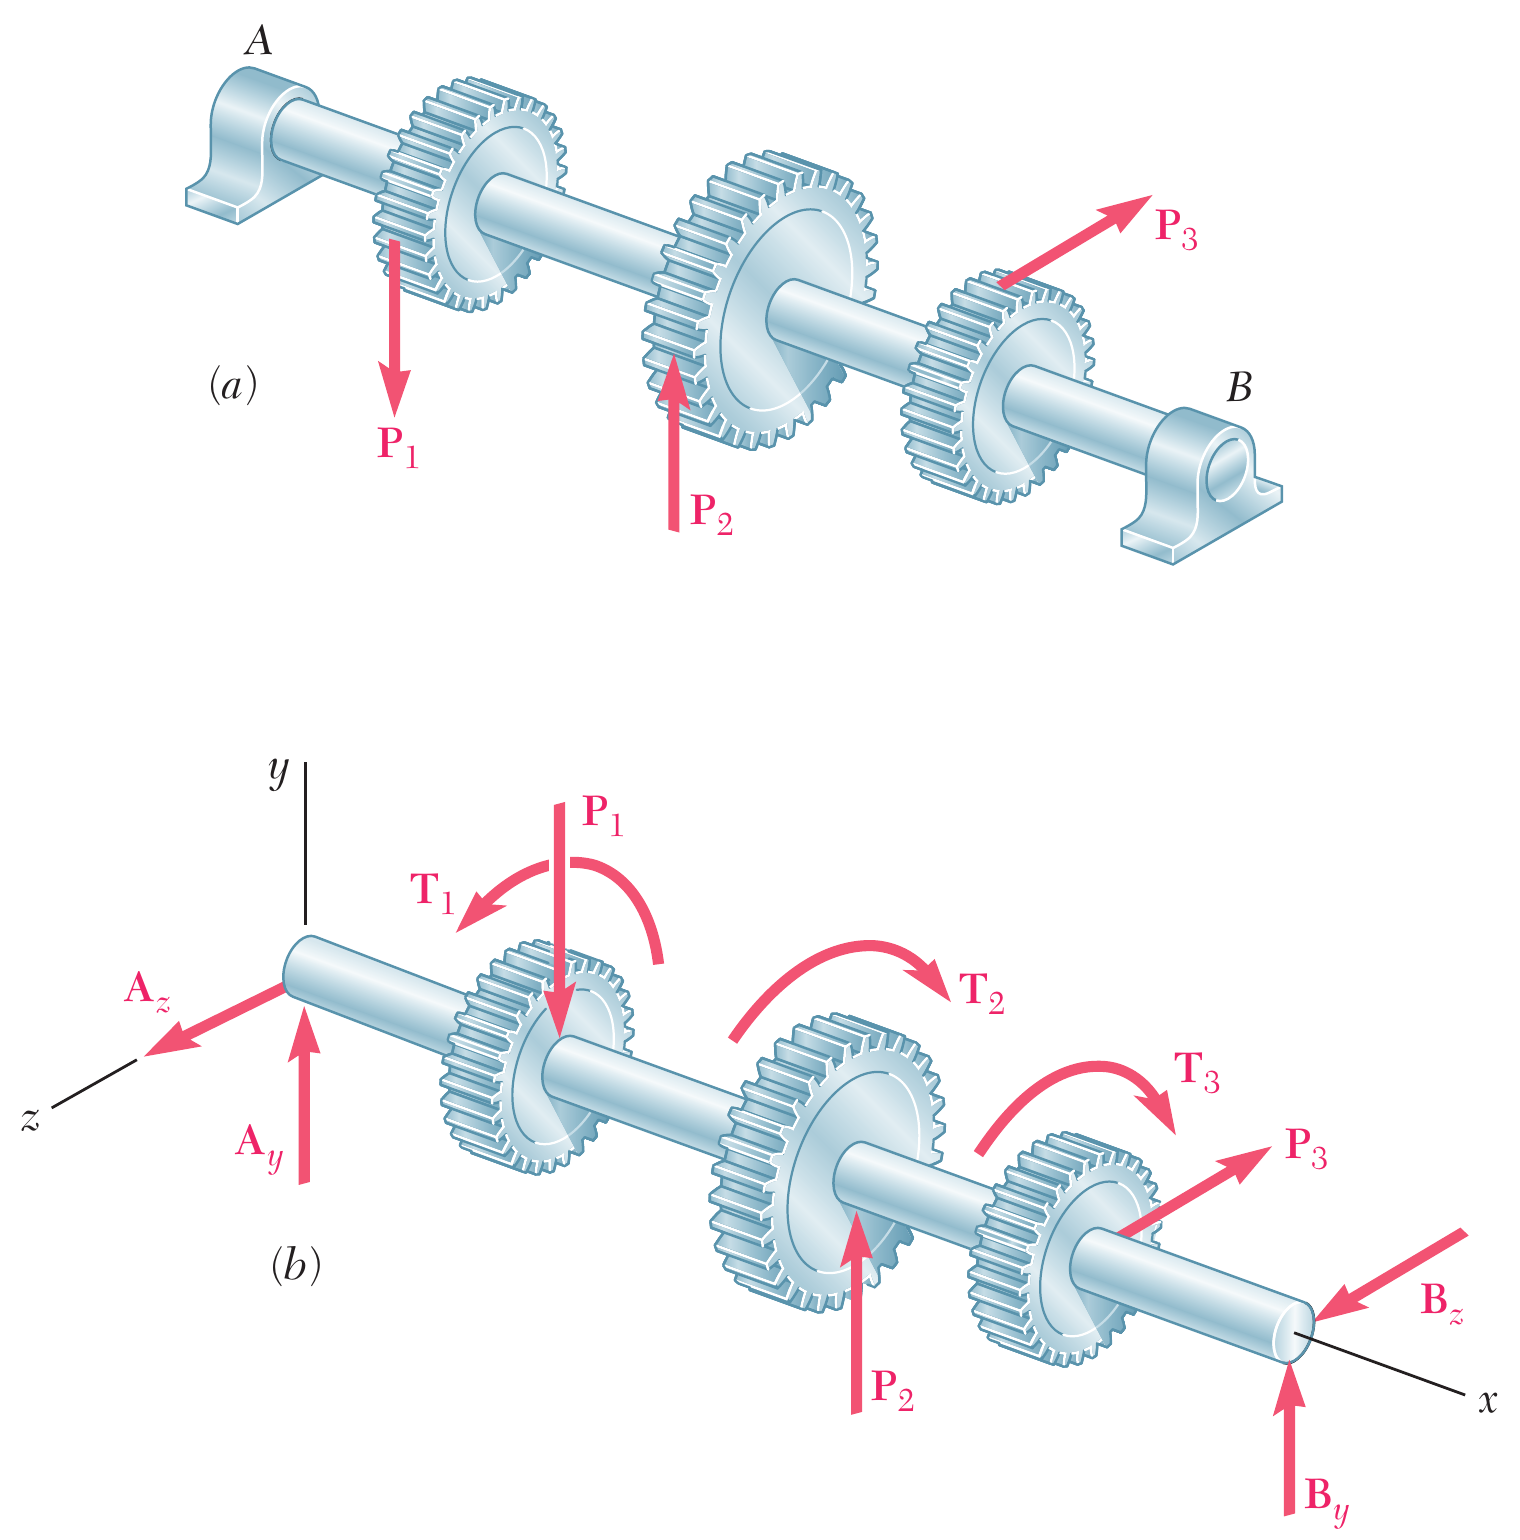
\includegraphics[width=\linewidth,height=5.5cm,keepaspectratio]{Chap_8/fig_8_11.png}
  \end{columns}
\end{frame}
% ===========
\begin{frame}[t]{Thiết kế trục truyền động (tiếp)}
  \begin{columns}[T]
    \column{0.60\textwidth}
      \small
      \begin{itemize}
        \setlength{\itemsep}{0.5em}
        \item Tại một mặt cắt bất kỳ:
        \[
          \sigma_m = \frac{Mc}{I} \quad\text{với}\quad M^2 = M_y^2 + M_z^2
          \qquad
          \tau_m = \frac{Tc}{J}
        \]
        \item Ứng suất tiếp lớn nhất:
        \[
          \tau_{\max} = \sqrt{\left(\frac{\sigma_m}{2}\right)^2 + (\tau_m)^2}
            = \sqrt{\left(\frac{Mc}{2I}\right)^2 + \left(\frac{Tc}{J}\right)^2}
        \]
        với mặt cắt tròn đặc hoặc tròn rỗng, $2I = J$:
        \[
          \tau_{\max} = \frac{c}{J}\sqrt{M^2 + T^2}
        \]
        \item Yêu cầu đối với mặt cắt trục:
        \[
          \left(\frac{J}{c}\right)_{\min}
            = \frac{\left(\sqrt{M^2 + T^2}\right)_{\max}}{\tau_{\mathrm{all}}}
        \]
      \end{itemize}
    \column{0.38\textwidth}
      \centering
      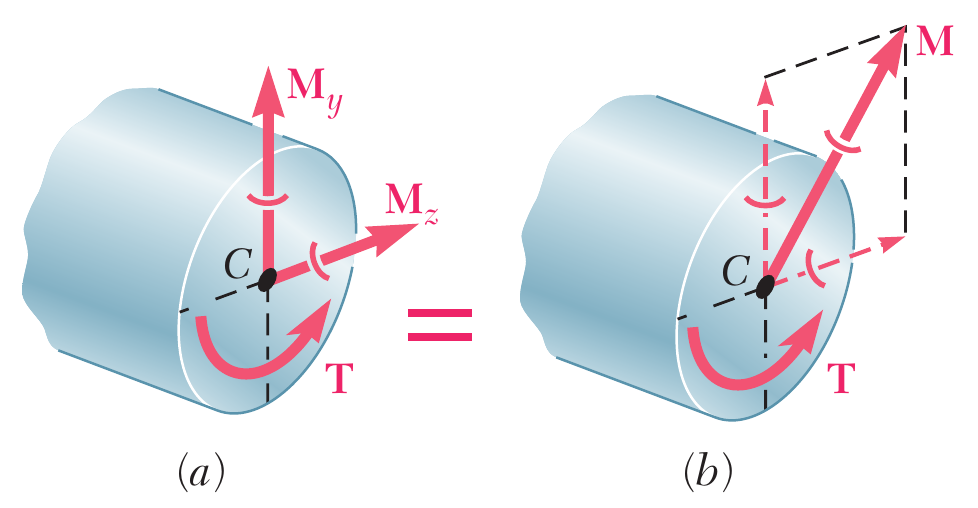
\includegraphics[width=\linewidth,height=2.9cm,keepaspectratio]{Chap_8/fig_8_12.png}\\[2pt]
      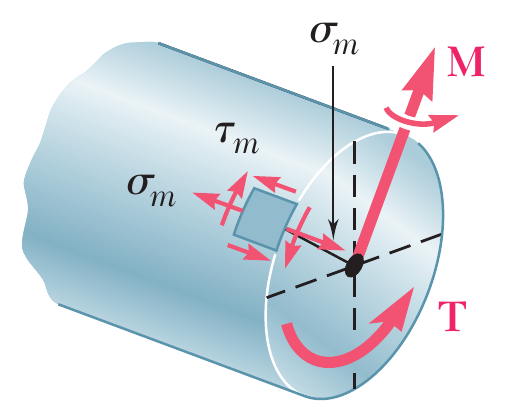
\includegraphics[width=\linewidth,height=2.9cm,keepaspectratio]{Chap_8/fig_8_13.png}
  \end{columns}
\end{frame}
% ===========
\section{Bài mẫu 8.3}
\begin{frame}[t]{Bài mẫu 8.3}
  \begin{columns}[T]
    \column{0.42\textwidth}
      \centering
      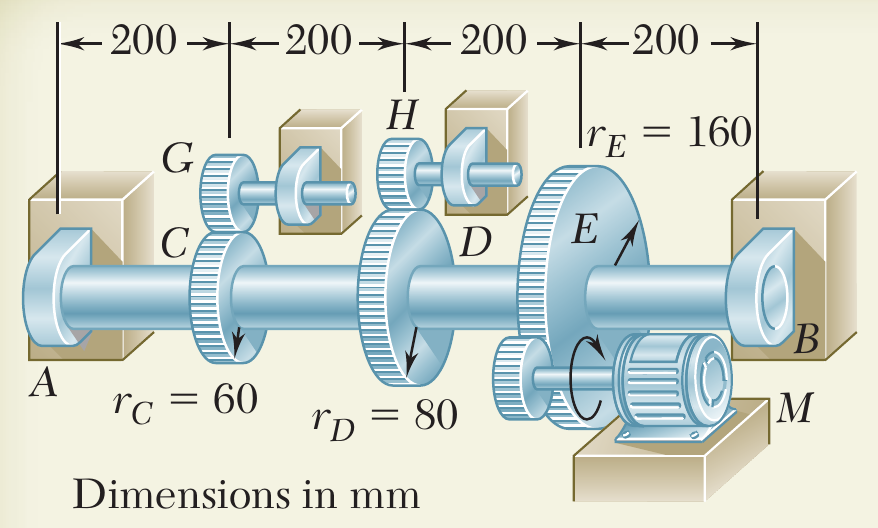
\includegraphics[width=\linewidth,height=5.5cm,keepaspectratio]{Chap_8/sp_8_3_a.png}
    \column{0.56\textwidth}
      \small
      Trục đặc quay với tốc độ 480 vòng/phút và truyền 30 kW từ động cơ đến
      các bánh răng $G$ và $H$; 20 kW được lấy ra tại bánh răng $G$ và 10 kW
      tại bánh răng $H$. Biết $\tau_{\mathrm{all}} = 50\,\mathrm{MPa}$, xác
      định đường kính nhỏ nhất cho phép của trục.

      \vspace{0.5em}
      \textbf{LỜI GIẢI:}
      \begin{itemize}
        \setlength{\itemsep}{0.3em}
        \item Xác định mô men xoắn trên các bánh răng và lực tiếp tuyến tương
              ứng.
        \item Tìm phản lực tại $A$ và $B$.
        \item Xác định mặt cắt nguy hiểm của trục từ các biểu đồ mô men xoắn
              và mô men uốn.
        \item Tính đường kính trục nhỏ nhất cho phép.
      \end{itemize}
  \end{columns}
\end{frame}
% ===========
\begin{frame}[t]{Bài mẫu 8.3 (tiếp)}
  \begin{columns}[T]
    \column{0.56\textwidth}
      \footnotesize
      \textbf{LỜI GIẢI:}
      \begin{itemize}
        \setlength{\itemsep}{0.20em}
        \item Xác định mô men xoắn trên các bánh răng và lực tiếp tuyến tương
              ứng:
        \[
          T_E = \frac{P}{2\pi f} = \frac{30\,\mathrm{kW}}{2\pi(8\,\mathrm{Hz})}
            = 597\,\mathrm{N\cdot m}
        \]
        \[
          F_E = \frac{T_E}{r_E} = \frac{597\,\mathrm{N\cdot m}}{0{,}16\,\mathrm{m}}
            = 3{,}73\,\mathrm{kN}
        \]
        \[
          T_C = \frac{20\,\mathrm{kW}}{2\pi(8\,\mathrm{Hz})} = 398\,\mathrm{N\cdot m}
          \qquad F_C = 6{,}63\,\mathrm{kN}
        \]
        \[
          T_D = \frac{10\,\mathrm{kW}}{2\pi(8\,\mathrm{Hz})} = 199\,\mathrm{N\cdot m}
          \qquad F_D = 2{,}49\,\mathrm{kN}
        \]
        \item Tìm phản lực tại $A$ và $B$:
        \[
          A_y = 0{,}932\,\mathrm{kN} \quad A_z = 6{,}22\,\mathrm{kN}
        \]
        \[
          B_y = 2{,}80\,\mathrm{kN} \quad B_z = 2{,}90\,\mathrm{kN}
        \]
      \end{itemize}
    \column{0.42\textwidth}
      \centering
      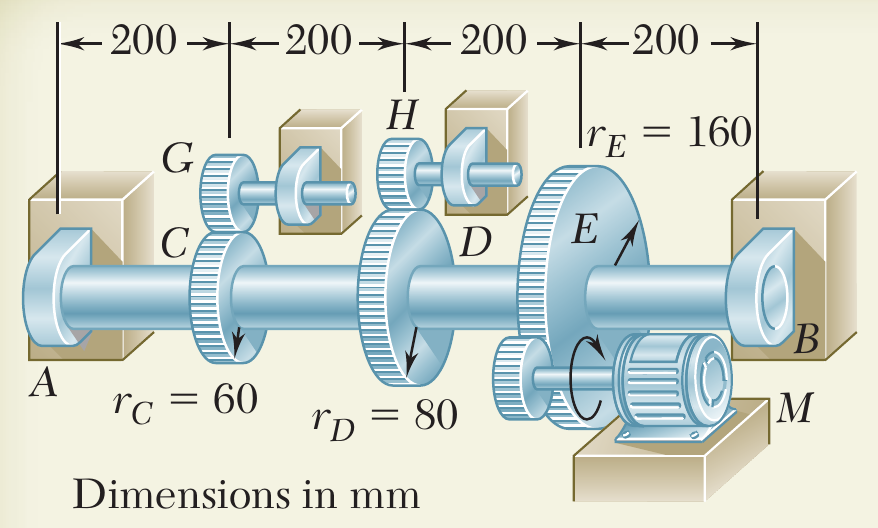
\includegraphics[width=\linewidth,height=4.7cm,keepaspectratio]{Chap_8/sp_8_3_a.png}
  \end{columns}
\end{frame}
% ===========
\begin{frame}[t]{Bài mẫu 8.3 (tiếp)}
  \begin{columns}[T]
    \column{0.40\textwidth}
      \small
      \begin{itemize}
        \setlength{\itemsep}{0.6em}
        \item Xác định mặt cắt nguy hiểm của trục từ các biểu đồ mô men xoắn
              và mô men uốn:
        \[
          \sqrt{M_y^2 + M_z^2 + T^2}_{\max} = 1357\,\mathrm{N\cdot m}
        \]
        \[
          T_{e,C} = 1319\,\mathrm{N\cdot m}
        \]
        \[
          T_{e,E} = 1003\,\mathrm{N\cdot m}
        \]
      \end{itemize}
    \column{0.58\textwidth}
      \centering
      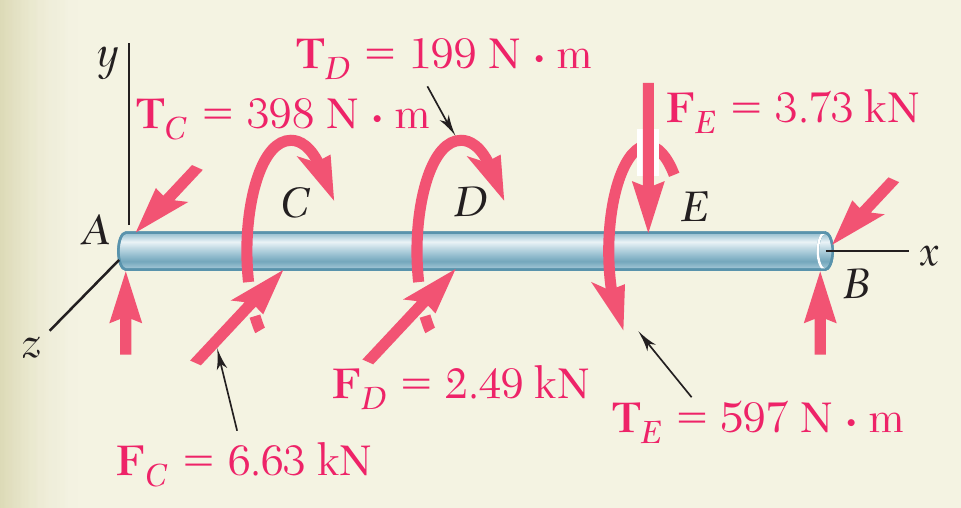
\includegraphics[width=\linewidth,height=6cm,keepaspectratio]{Chap_8/sp_8_3_b.png}
  \end{columns}
\end{frame}
% ===========
\begin{frame}[t]{Bài mẫu 8.3 (tiếp)}
  \begin{columns}[T]
    \column{0.56\textwidth}
      \small
      \begin{itemize}
        \setlength{\itemsep}{0.6em}
        \item Tính đường kính trục nhỏ nhất cho phép:
        \[
          \frac{J}{c} = \frac{\sqrt{M_y^2 + M_z^2 + T^2}}{\tau_{\mathrm{all}}}
            = \frac{1357\,\mathrm{N\cdot m}}{50\,\mathrm{MPa}}
        \]
        \[
          \frac{J}{c} = 27{,}14\times10^{-6}\,\mathrm{m}^3
        \]
        Với trục tròn đặc:
        \[
          \frac{J}{c} = \frac{\pi}{2}c^3 = 27{,}14\times10^{-6}\,\mathrm{m}^3
        \]
        \[
          c = 0{,}02585\,\mathrm{m} = 25{,}85\,\mathrm{mm}
        \]
        \[
          \boxed{d = 2c = 51{,}7\,\mathrm{mm}}
        \]
      \end{itemize}
    \column{0.42\textwidth}
      \centering
      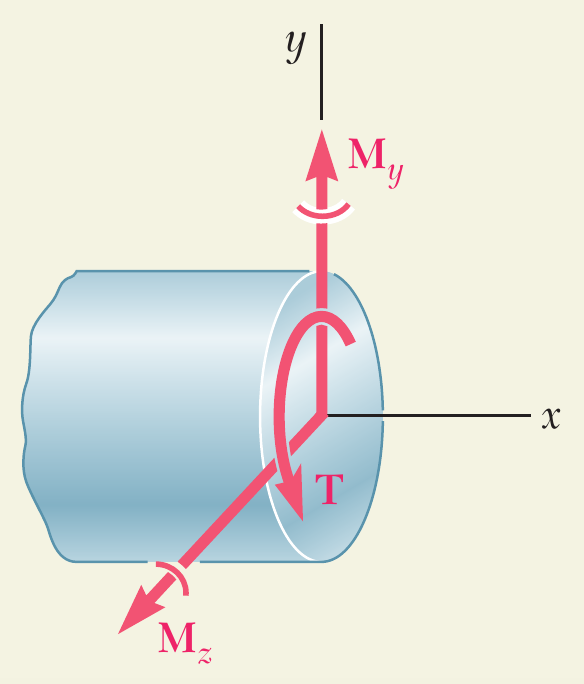
\includegraphics[width=\linewidth,height=5.5cm,keepaspectratio]{Chap_8/sp_8_3_c.png}
  \end{columns}
\end{frame}
% ===========
\section{Ứng suất dưới tác dụng của tải trọng tổ hợp}
\begin{frame}[t]{Ứng suất dưới tác dụng của tải trọng tổ hợp}
  \begin{columns}[T]
    \column{0.56\textwidth}
      \small
      \begin{itemize}
        \setlength{\itemsep}{0.7em}
        \item Cần xác định ứng suất trong các cấu kiện mảnh chịu tải trọng bất
              kỳ.
        \item Cắt qua các điểm cần khảo sát. Xác định hệ lực -- ngẫu lực tại
              trọng tâm mặt cắt cần thiết để duy trì cân bằng.
        \item Hệ nội lực gồm ba thành phần lực và ba véc tơ ngẫu lực.
        \item Xác định phân bố ứng suất bằng cách áp dụng nguyên lý cộng tác
              dụng.
      \end{itemize}
    \column{0.42\textwidth}
      \centering
      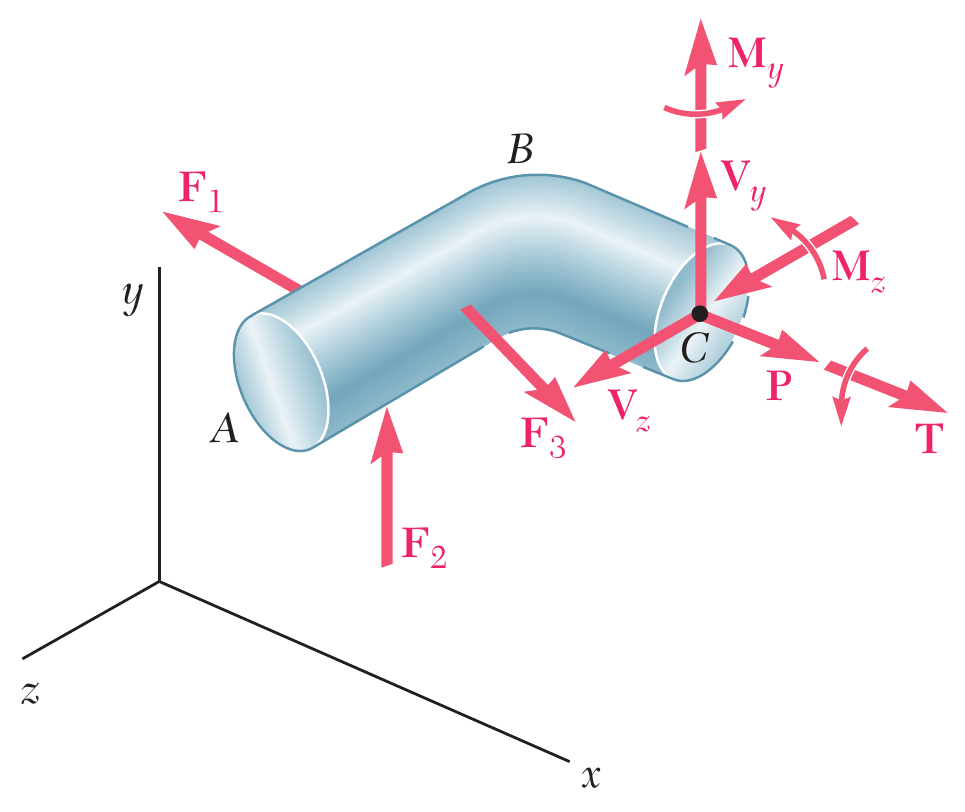
\includegraphics[width=\linewidth,height=2.9cm,keepaspectratio]{Chap_8/fig_8_16.png}\\[2pt]
      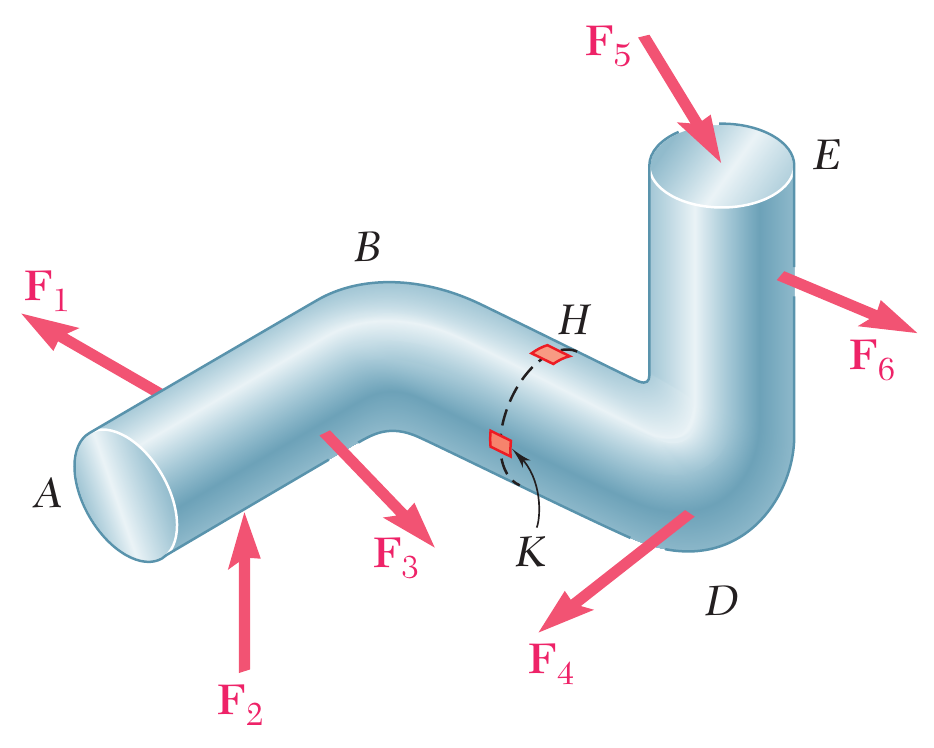
\includegraphics[width=\linewidth,height=2.9cm,keepaspectratio]{Chap_8/fig_8_15.png}
  \end{columns}
\end{frame}
% ===========
\begin{frame}[t]{Ứng suất dưới tác dụng của tải trọng tổ hợp (tiếp)}
  \begin{columns}[T]
    \column{0.50\textwidth}
      \small
      \begin{itemize}
        \setlength{\itemsep}{1em}
        \item Lực dọc trục và các véc tơ ngẫu lực nằm trong mặt phẳng mặt cắt
              (mô men uốn) đóng góp vào phân bố ứng suất pháp trên mặt cắt.
        \item Các thành phần lực cắt và ngẫu lực xoắn đóng góp vào phân bố ứng
              suất tiếp trên mặt cắt.
      \end{itemize}
    \column{0.48\textwidth}
      \centering
      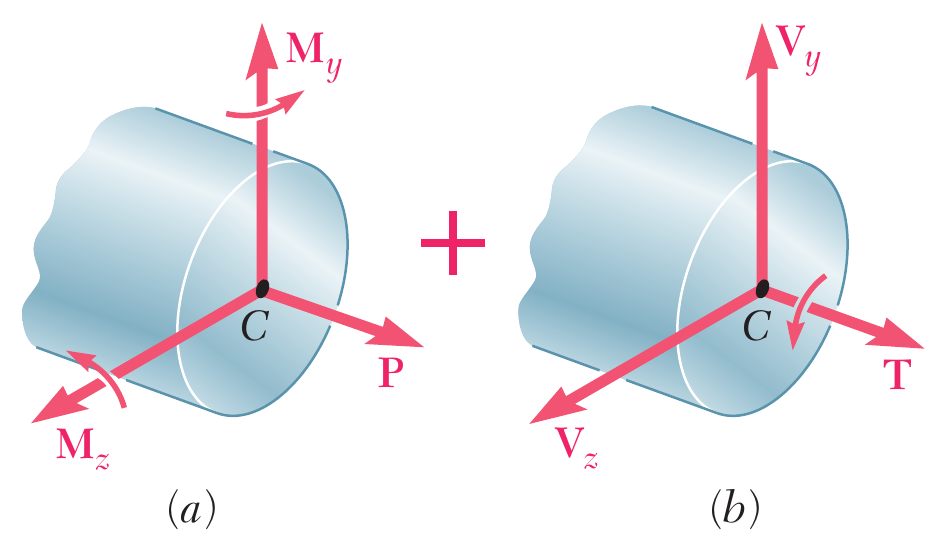
\includegraphics[width=\linewidth,height=2.9cm,keepaspectratio]{Chap_8/fig_8_17.png}\\[2pt]
      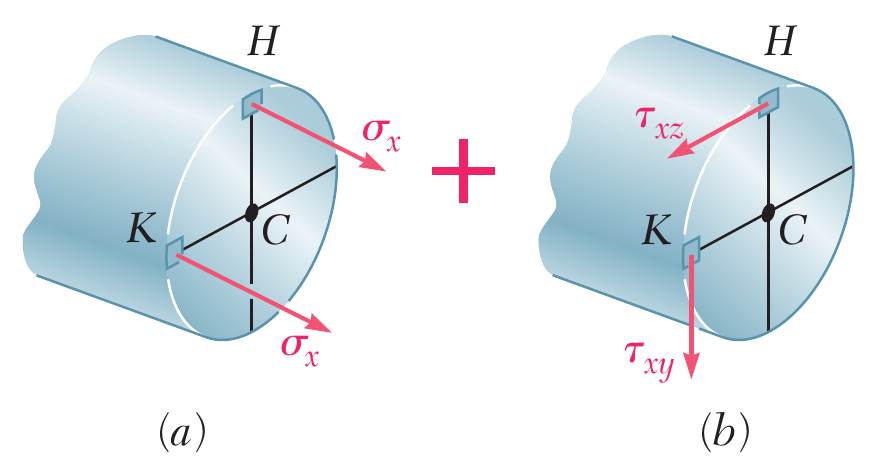
\includegraphics[width=\linewidth,height=2.9cm,keepaspectratio]{Chap_8/fig_8_18.png}
  \end{columns}
\end{frame}
% ===========
\begin{frame}[t]{Ứng suất dưới tác dụng của tải trọng tổ hợp (tiếp)}
  \begin{columns}[T]
    \column{0.52\textwidth}
      \small
      \begin{itemize}
        \setlength{\itemsep}{1em}
        \item Ứng suất pháp và ứng suất tiếp được dùng để xác định các ứng suất
              chính, ứng suất tiếp lớn nhất và hướng của các mặt chính.
        \item Phân tích chỉ đúng trong phạm vi các điều kiện áp dụng của
              nguyên lý cộng tác dụng và nguyên lý Saint-Venant được thỏa mãn.
      \end{itemize}
    \column{0.46\textwidth}
      \centering
      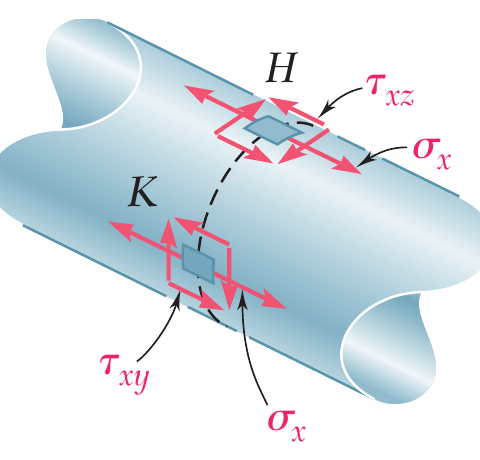
\includegraphics[width=\linewidth,height=5.5cm,keepaspectratio]{Chap_8/fig_8_19.png}
  \end{columns}
\end{frame}
% ===========
\section{Bài mẫu 8.5}
\begin{frame}[t]{Bài mẫu 8.5}
  \begin{columns}[T]
    \column{0.42\textwidth}
      \centering
      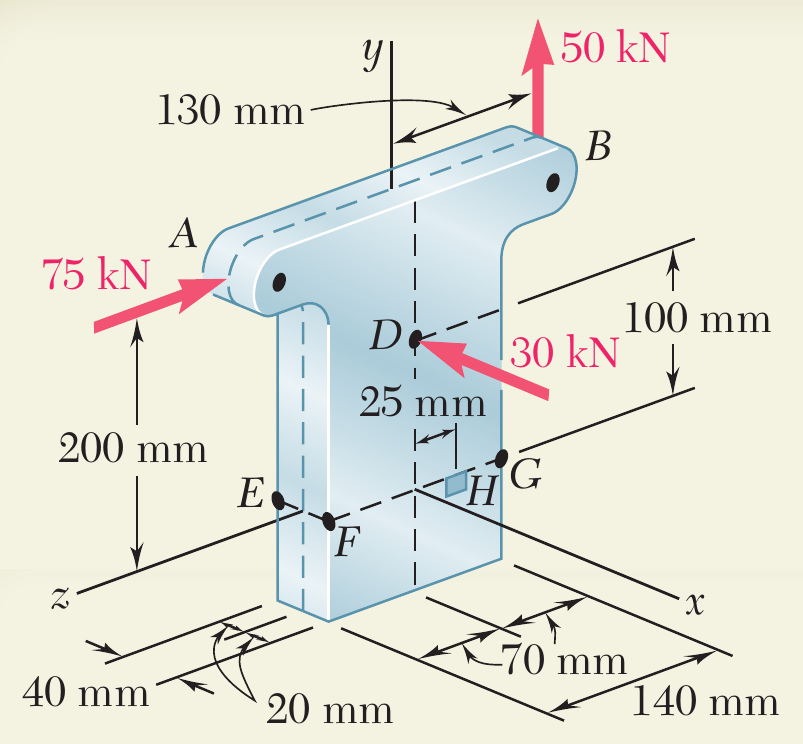
\includegraphics[width=\linewidth,height=5.5cm,keepaspectratio]{Chap_8/sp_8_5_a.png}
    \column{0.56\textwidth}
      \small
      Ba lực tác dụng lên một cột thép ngắn như hình vẽ. Xác định các ứng
      suất chính, các mặt chính và ứng suất tiếp lớn nhất tại điểm $H$.

      \vspace{0.8em}
      \textbf{LỜI GIẢI:}
      \begin{itemize}
        \setlength{\itemsep}{0.4em}
        \item Xác định nội lực tại mặt cắt $EFG$.
        \item Tính ứng suất pháp tại $H$.
        \item Tính ứng suất tiếp tại $H$.
        \item Tính các ứng suất chính và ứng suất tiếp lớn nhất. Xác định các
              mặt chính.
      \end{itemize}
  \end{columns}
\end{frame}
% ===========
\begin{frame}[t]{Bài mẫu 8.5 (tiếp)}
  \begin{columns}[T]
    \column{0.58\textwidth}
      \small
      \textbf{LỜI GIẢI:}
      \begin{itemize}
        \setlength{\itemsep}{0.4em}
        \item Xác định nội lực tại mặt cắt $EFG$:
        \[
          V_x = -30\,\mathrm{kN} \qquad P = 50\,\mathrm{kN} \qquad
          V_z = -75\,\mathrm{kN}
        \]
        \[
          M_x = (50)(0{,}130) - (75)(0{,}200) = -8{,}5\,\mathrm{kN\cdot m}
        \]
        \[
          M_y = 0 \qquad M_z = (30\,\mathrm{kN})(0{,}100\,\mathrm{m}) = 3\,\mathrm{kN\cdot m}
        \]
      \end{itemize}
      Lưu ý: Các đặc trưng mặt cắt
      \[
        A = (0{,}040\,\mathrm{m})(0{,}140\,\mathrm{m}) = 5{,}6\times10^{-3}\,\mathrm{m}^2
      \]
      \[
        I_x = \tfrac{1}{12}(0{,}040\,\mathrm{m})(0{,}140\,\mathrm{m})^3 = 9{,}15\times10^{-6}\,\mathrm{m}^4
      \]
      \[
        I_z = \tfrac{1}{12}(0{,}140\,\mathrm{m})(0{,}040\,\mathrm{m})^3 = 0{,}747\times10^{-6}\,\mathrm{m}^4
      \]
    \column{0.40\textwidth}
      \centering
      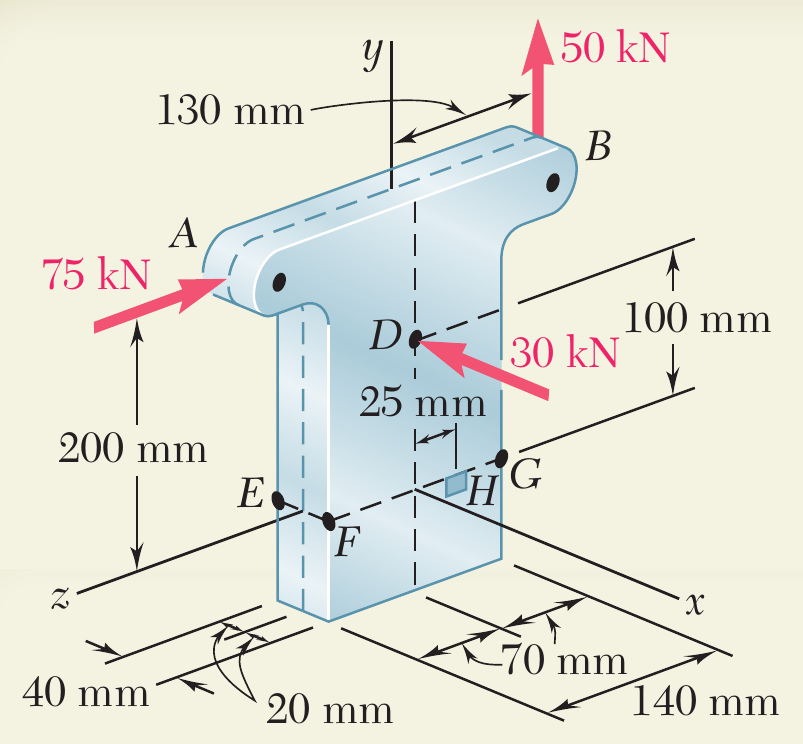
\includegraphics[width=\linewidth,height=5.5cm,keepaspectratio]{Chap_8/sp_8_5_a.png}
  \end{columns}
\end{frame}
% ===========
\begin{frame}[t]{Bài mẫu 8.5 (tiếp)}
  \begin{columns}[T]
    \column{0.60\textwidth}
      \small
      \begin{itemize}
        \setlength{\itemsep}{0.5em}
        \item Tính ứng suất pháp tại $H$:
        \[
          \sigma_y = +\frac{P}{A} + \frac{|M_z|a}{I_z} - \frac{|M_x|b}{I_x}
        \]
        \[
          = \frac{50\,\mathrm{kN}}{5{,}6\times10^{-3}}
            + \frac{(3\,\mathrm{kN\cdot m})(0{,}020)}{0{,}747\times10^{-6}}
            - \frac{(8{,}5\,\mathrm{kN\cdot m})(0{,}025)}{9{,}15\times10^{-6}}
        \]
        \[
          = (8{,}93 + 80{,}3 - 23{,}2)\,\mathrm{MPa} = 66{,}0\,\mathrm{MPa}
        \]
        \item Tính ứng suất tiếp tại $H$:
        \[
          Q = A_1\bar{y}_1 = \left[(0{,}040)(0{,}045)\right](0{,}0475)
            = 85{,}5\times10^{-6}\,\mathrm{m}^3
        \]
        \[
          \tau_{yz} = \frac{V_zQ}{I_xt}
            = \frac{(75\,\mathrm{kN})(85{,}5\times10^{-6})}{(9{,}15\times10^{-6})(0{,}040)}
            = 17{,}52\,\mathrm{MPa}
        \]
      \end{itemize}
    \column{0.38\textwidth}
      \centering
      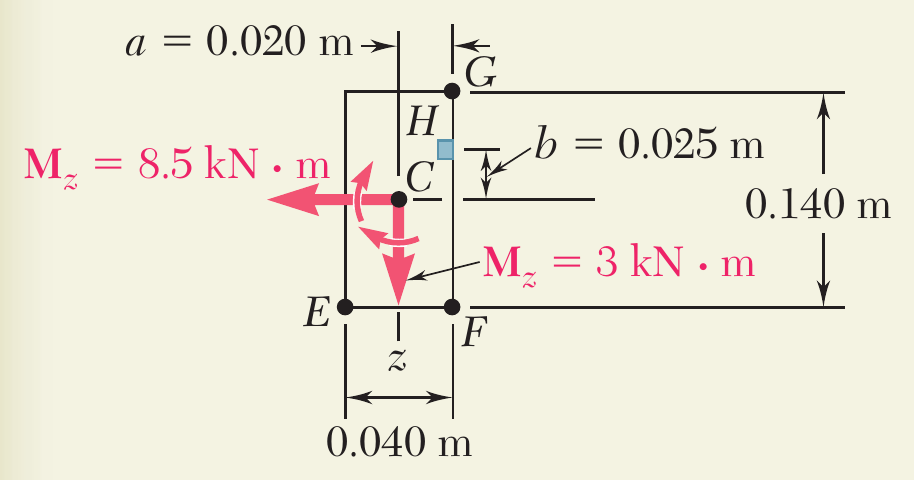
\includegraphics[width=\linewidth,height=2.9cm,keepaspectratio]{Chap_8/sp_8_5_b.png}\\[2pt]
      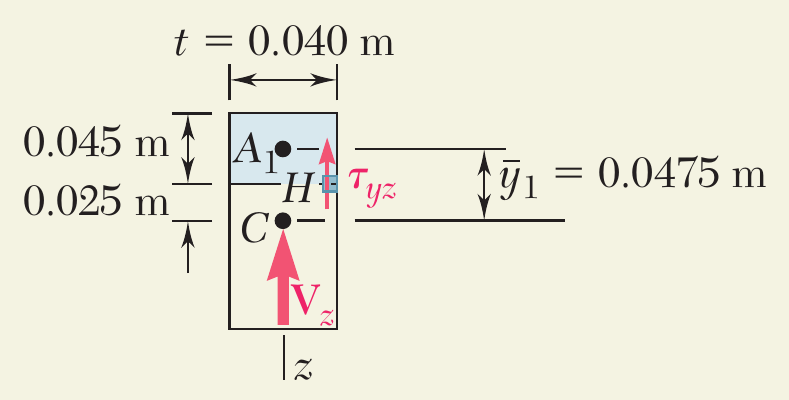
\includegraphics[width=\linewidth,height=2.9cm,keepaspectratio]{Chap_8/sp_8_5_c.png}
  \end{columns}
\end{frame}
% ===========
\begin{frame}[t]{Bài mẫu 8.5 (tiếp)}
  \begin{columns}[T]
    \column{0.56\textwidth}
      \small
      \begin{itemize}
        \setlength{\itemsep}{0.4em}
        \item Tính các ứng suất chính và ứng suất tiếp lớn nhất. Xác định các
              mặt chính:
        \[
          \tau_{\max} = R = \sqrt{33{,}0^2 + 17{,}52^2} = 37{,}4\,\mathrm{MPa}
        \]
        \[
          \sigma_{\max} = OC + R = 33{,}0 + 37{,}4 = 70{,}4\,\mathrm{MPa}
        \]
        \[
          \sigma_{\min} = OC - R = 33{,}0 - 37{,}4 = -7{,}4\,\mathrm{MPa}
        \]
        \[
          \tan2\theta_p = \frac{CY}{CD} = \frac{17{,}52}{33{,}0}
        \]
        \[
          2\theta_p = 27{,}96^\circ \qquad \theta_p = 13{,}98^\circ
        \]
        \[
          \boxed{\tau_{\max} = 37{,}4\,\mathrm{MPa} \quad
                 \sigma_{\max} = 70{,}4\,\mathrm{MPa}}
        \]
        \[
          \boxed{\sigma_{\min} = -7{,}4\,\mathrm{MPa} \quad
                 \theta_p = 13{,}98^\circ}
        \]
      \end{itemize}
    \column{0.42\textwidth}
      \centering
      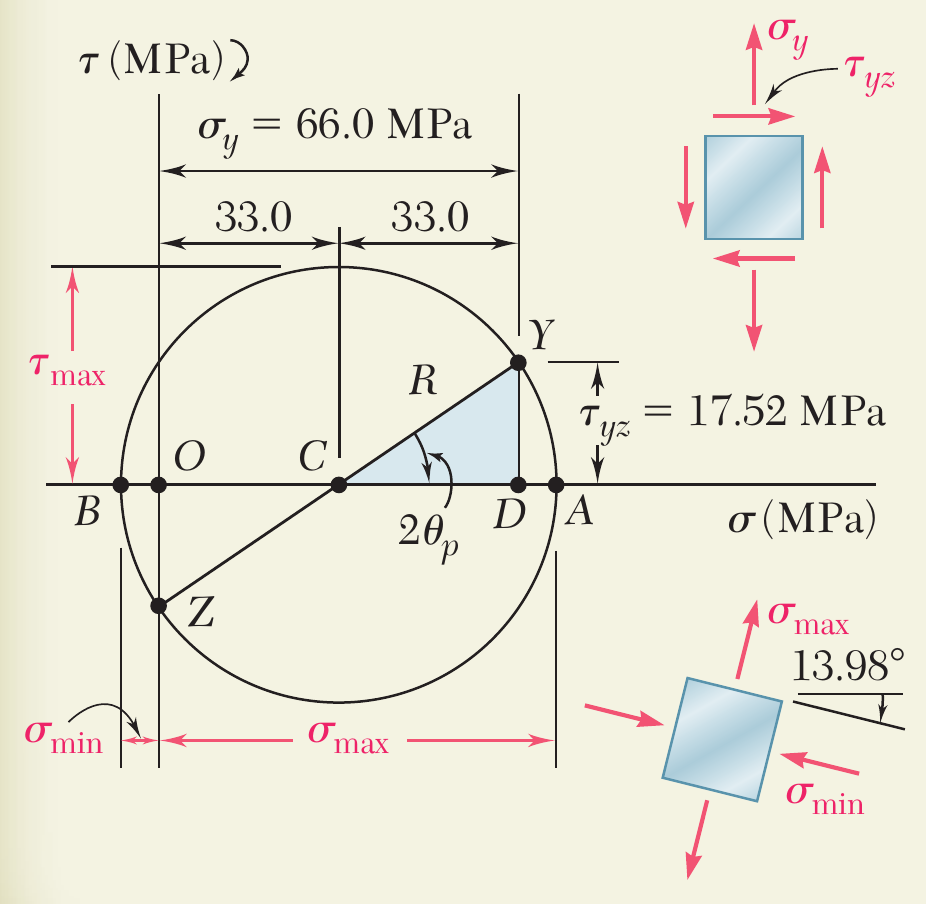
\includegraphics[width=\linewidth,height=2.9cm,keepaspectratio]{Chap_8/sp_8_5_d.png}\\[2pt]
      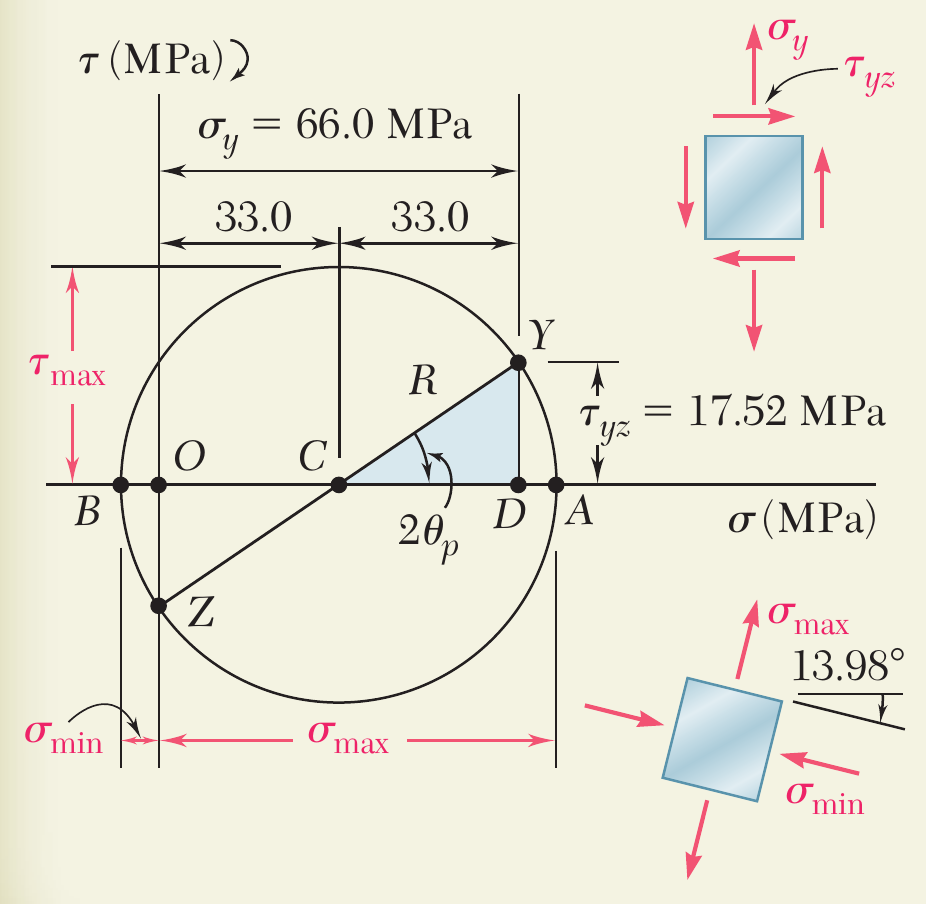
\includegraphics[width=\linewidth,height=2.9cm,keepaspectratio]{Chap_8/sp_8_5_d.png}
  \end{columns}
\end{frame}

\end{document}
